% Chapter 5
\chapter{Exploratory Data Analysis and Visualizations}
\label{ch:eda}

The exploratory analysis asks a narrow question: which observable behaviours at the grant date separate loans that were repaid from loans that ran into difficulty? The analysis is descriptive. No feature is selected or transformed on the basis of the target in a way that later leaks into the model. The figures in this chapter are produced from the same 682-row feature table used for modelling.

\section{Class Distribution}
\label{sec:class-distribution}

Figure~\ref{fig:target-dist} shows the target distribution. The dataset contains 606 good loans and 76 defaults, an 11.14\% default rate. The imbalance is moderate in absolute terms but severe enough that a majority-class predictor would reach 88.86\% accuracy while identifying no defaults. Every later evaluation therefore reports recall, F1, average precision, and ROC-AUC alongside accuracy.

\begin{figure}[H]
    \centering
    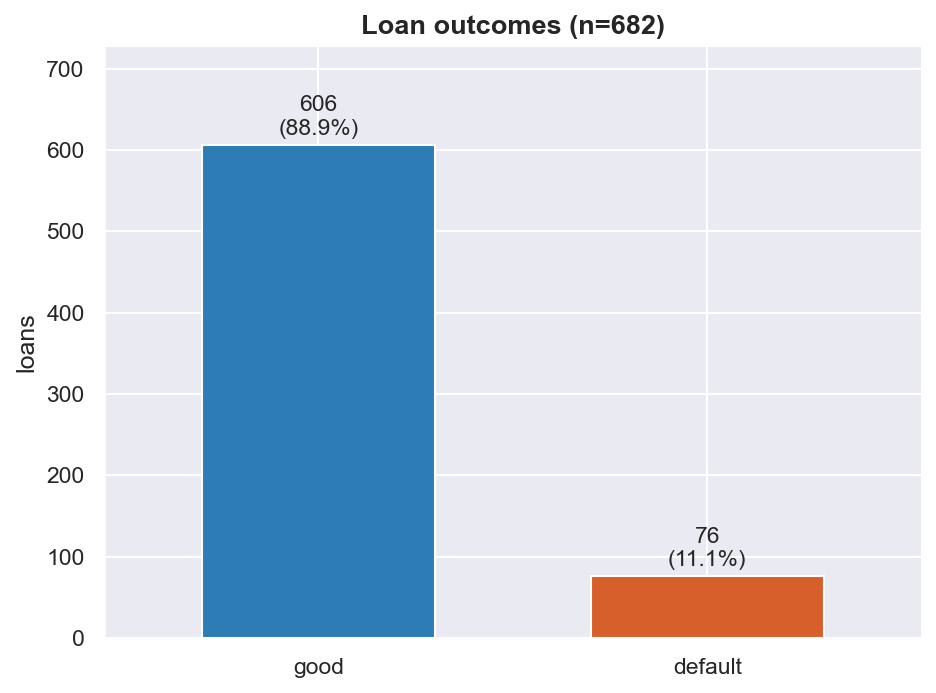
\includegraphics[width=0.62\textwidth]{target_dist.png}
    \caption{Distribution of the binary target: 606 good loans and 76 defaults (11.14\%).}
    \label{fig:target-dist}
\end{figure}

\section{Features Associated with Default}
\label{sec:target-correlations}

Figure~\ref{fig:corr-target} ranks the numeric features by their Pearson correlation with the default label. The strongest associations are negative and involve account balance: \texttt{min\_balance} at $-0.26$, \texttt{balance\_at\_loan} at $-0.20$, and \texttt{avg\_balance} at $-0.16$. Borrowers who defaulted tended to have lower balances before the loan, and the lowest point of their balance history was further below zero than for good borrowers.

On the loan side, \texttt{amount} correlates at $+0.17$ and \texttt{payments} at $+0.18$: larger loans and the higher monthly payments that come with them are associated with default. Age and gender are close to zero ($+0.01$ and $+0.02$), which is an early indication that the demographic variables carry little signal in this dataset.

\begin{figure}[H]
    \centering
    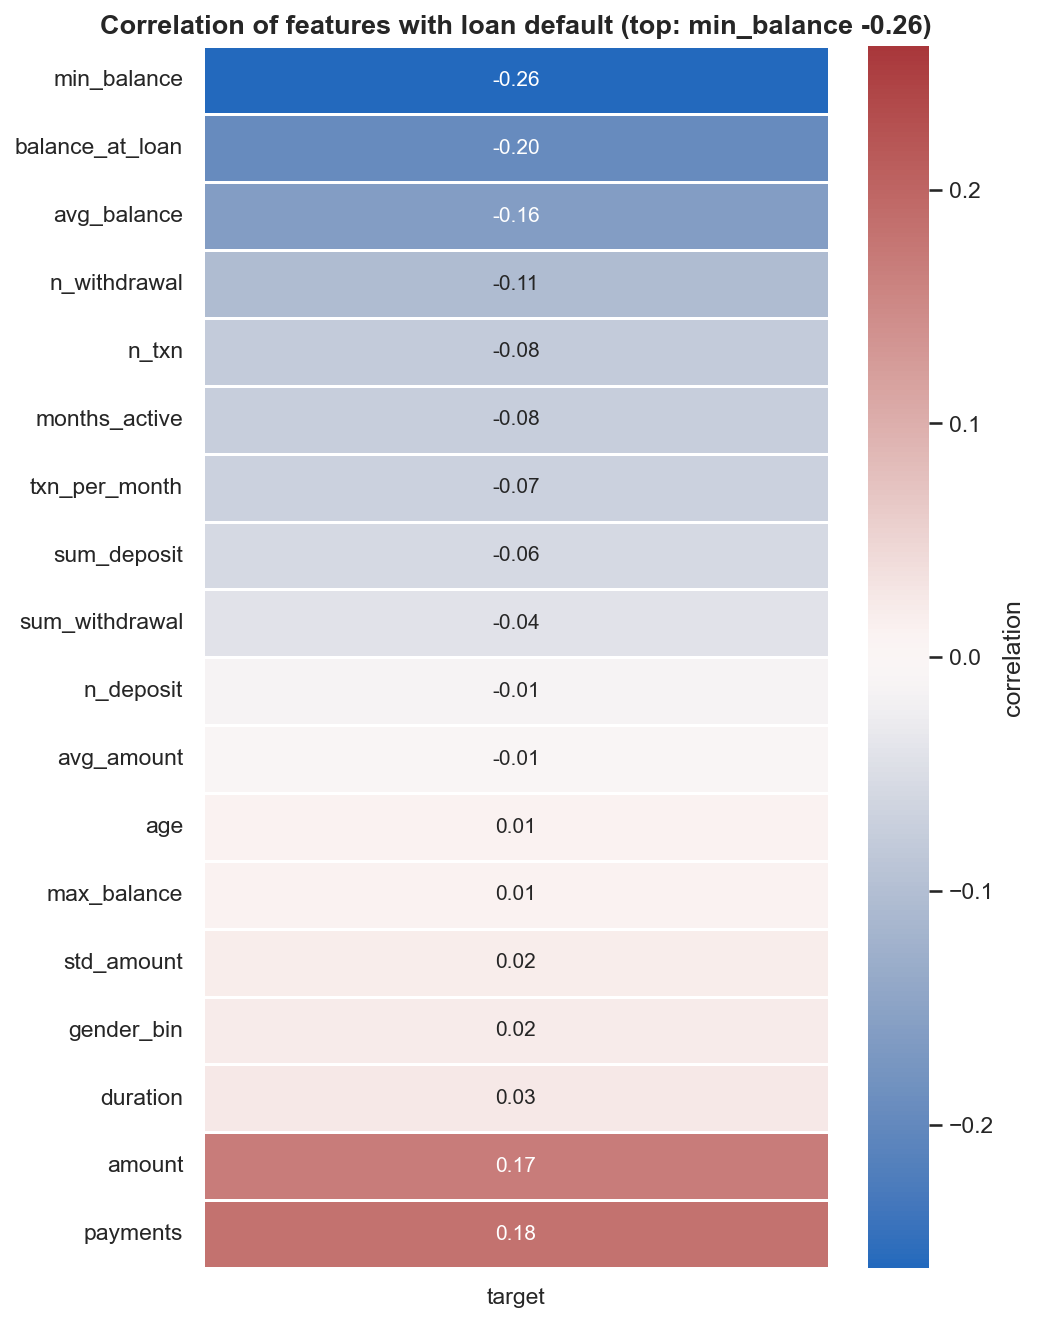
\includegraphics[width=0.62\textwidth]{corr_target.png}
    \caption{Correlation of each numeric feature with the default label. Balance features are negative; loan size and payment are positive.}
    \label{fig:corr-target}
\end{figure}

Correlation is a linear summary and can understate a relationship that is concentrated in a tail. The next two sections look at distributions rather than coefficients.

\section{Balance Separation}
\label{sec:balance-separation}

Figure~\ref{fig:behavior-box} compares the distributions of the main behavioural features for good and defaulted loans. The medians tell a consistent story. The balance at the loan date has a median of about 39,500 for good loans and 22,000 for defaults. Average balance is about 44,100 for good loans and 37,000 for defaults. The gap is not a handful of extreme accounts: the default distribution sits lower across its middle.

Transaction frequency barely separates the classes. Both groups transact at roughly 5.6 to 5.7 times per month. A busy account is not automatically a safe account. What matters more is the level of the balance and whether it was falling before the loan.

\begin{figure}[H]
    \centering
    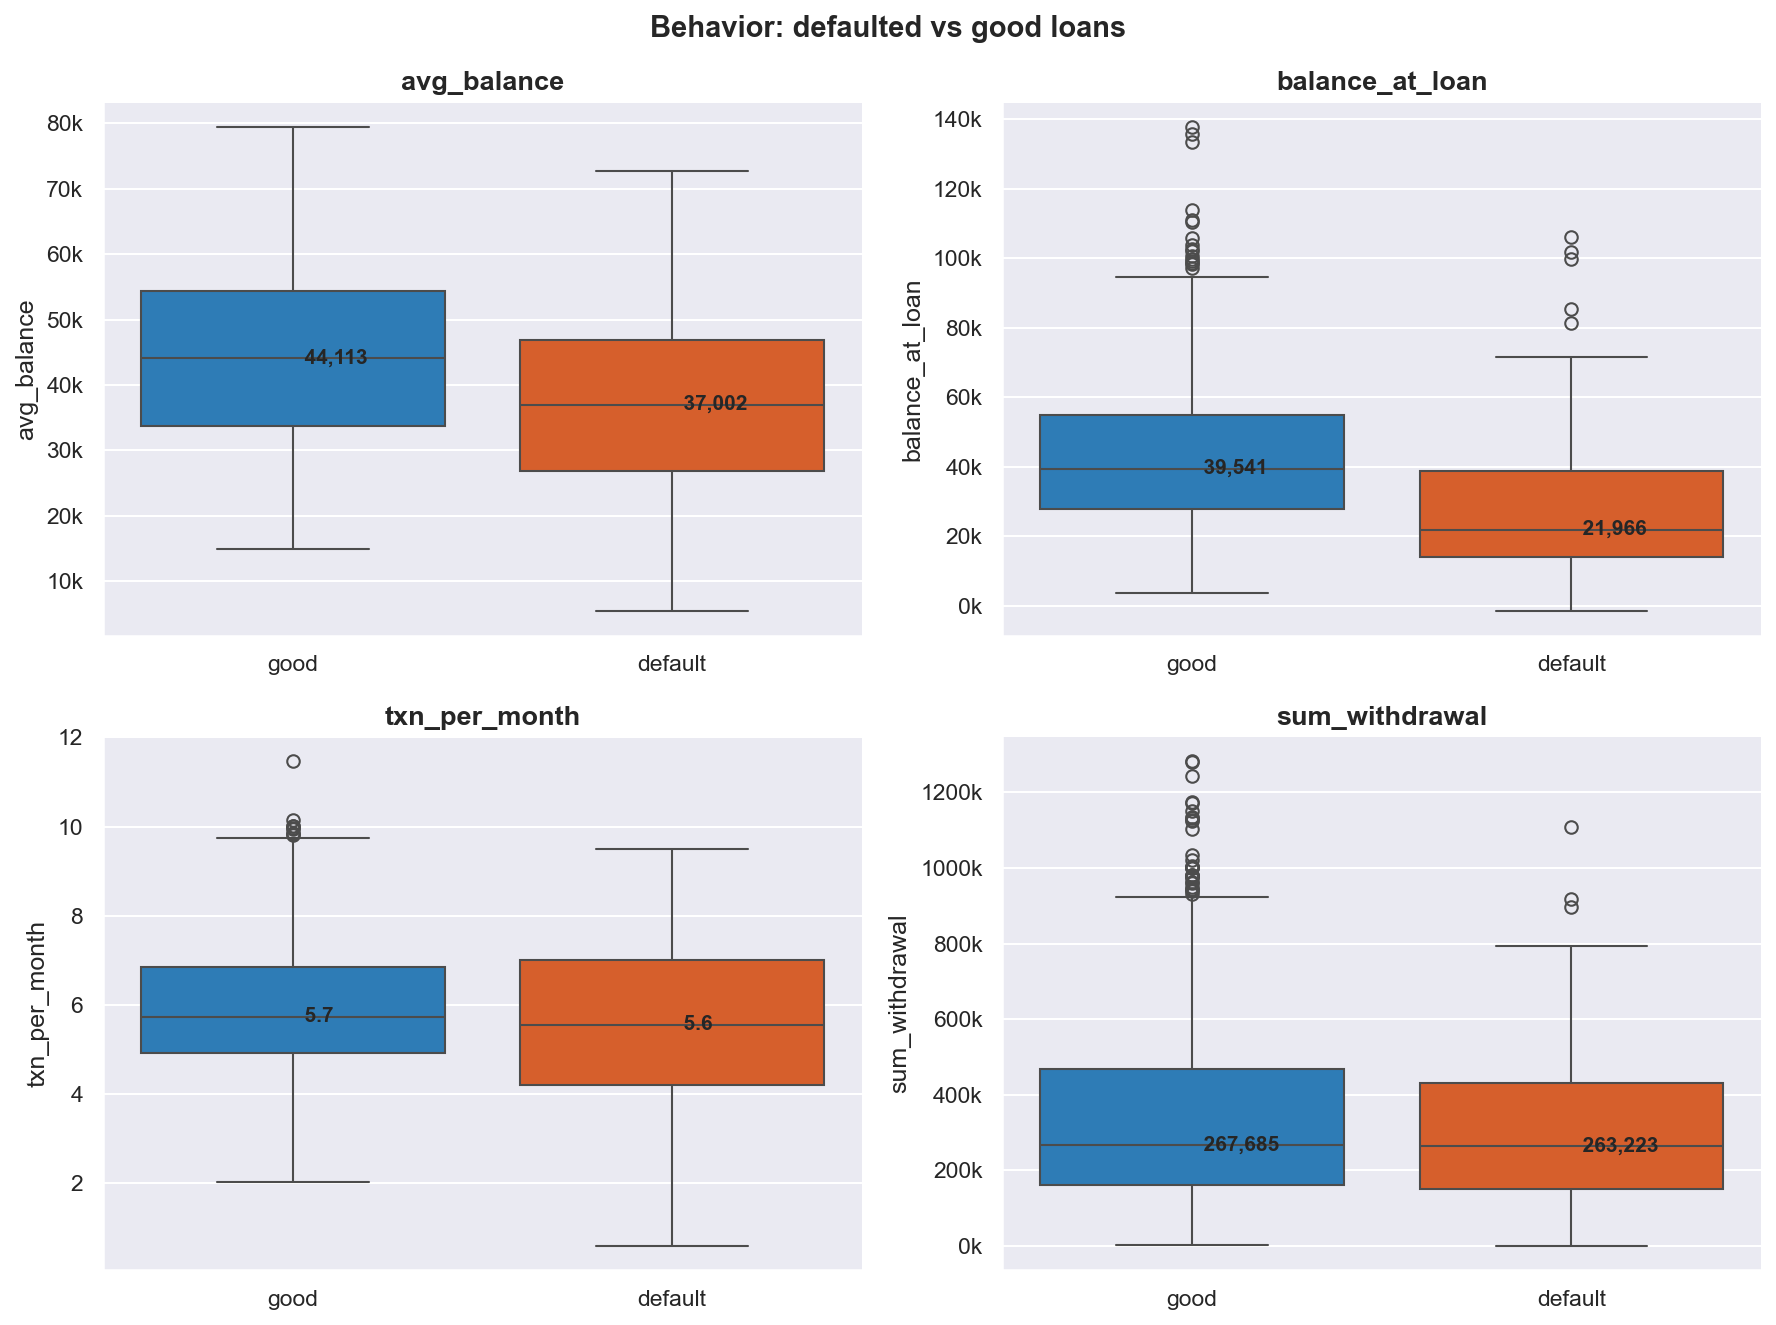
\includegraphics[width=0.9\textwidth]{behavior_box.png}
    \caption{Box plots of selected behavioural features by class. The balance distributions separate more clearly than transaction frequency.}
    \label{fig:behavior-box}
\end{figure}

\section{Age and Gender}
\label{sec:age-gender}

Figure~\ref{fig:age-hist} shows the age distribution split by outcome. Defaults appear across the full age range, with no concentration in a particular decade. The visual impression matches the near-zero correlation: age is not a useful discriminator on its own.

The gender split is similarly weak. Female borrowers default at 11.8\% and male borrowers at 10.5\%, a difference of 1.3 percentage points on a small minority class. With 76 defaults in total, that difference is well within sampling noise. Gender is kept as a feature for completeness, but the report does not build a business rule around it.

\begin{figure}[H]
    \centering
    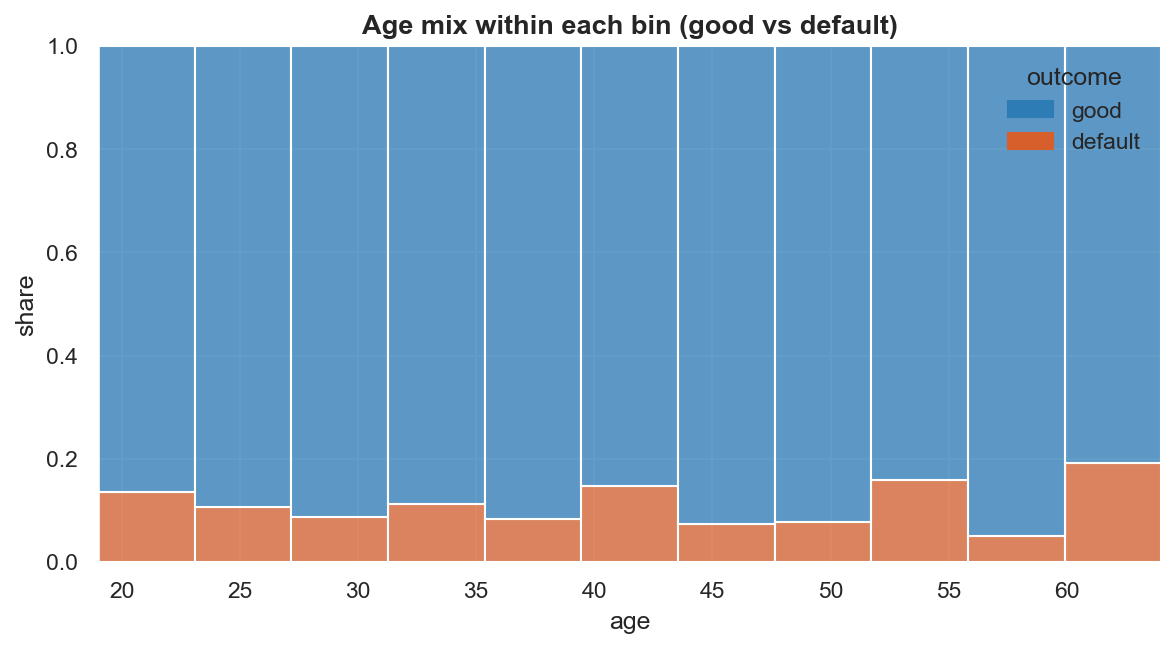
\includegraphics[width=0.75\textwidth]{age_hist.png}
    \caption{Age distribution by outcome. Defaults occur across all ages rather than in a single band.}
    \label{fig:age-hist}
\end{figure}

\section{Collinearity and Redundancy}
\label{sec:collinearity}

Figure~\ref{fig:corr-full} shows the full correlation matrix of the numeric features. Two clusters stand out. The first is the cash-flow pair: \texttt{sum\_deposit} and \texttt{sum\_withdrawal} correlate at 0.997, which is close to a duplicate. The second is the loan-burden pair: \texttt{amount} and \texttt{payments} move together, as they must under a fixed rate and duration.

The balance features form a softer cluster. \texttt{avg\_balance}, \texttt{min\_balance}, \texttt{max\_balance}, and \texttt{balance\_at\_loan} are related but not interchangeable; the minimum captures a different part of the distribution than the last observed value. This is why all four are retained, even though their importance scores will partly overlap.

\begin{figure}[H]
    \centering
    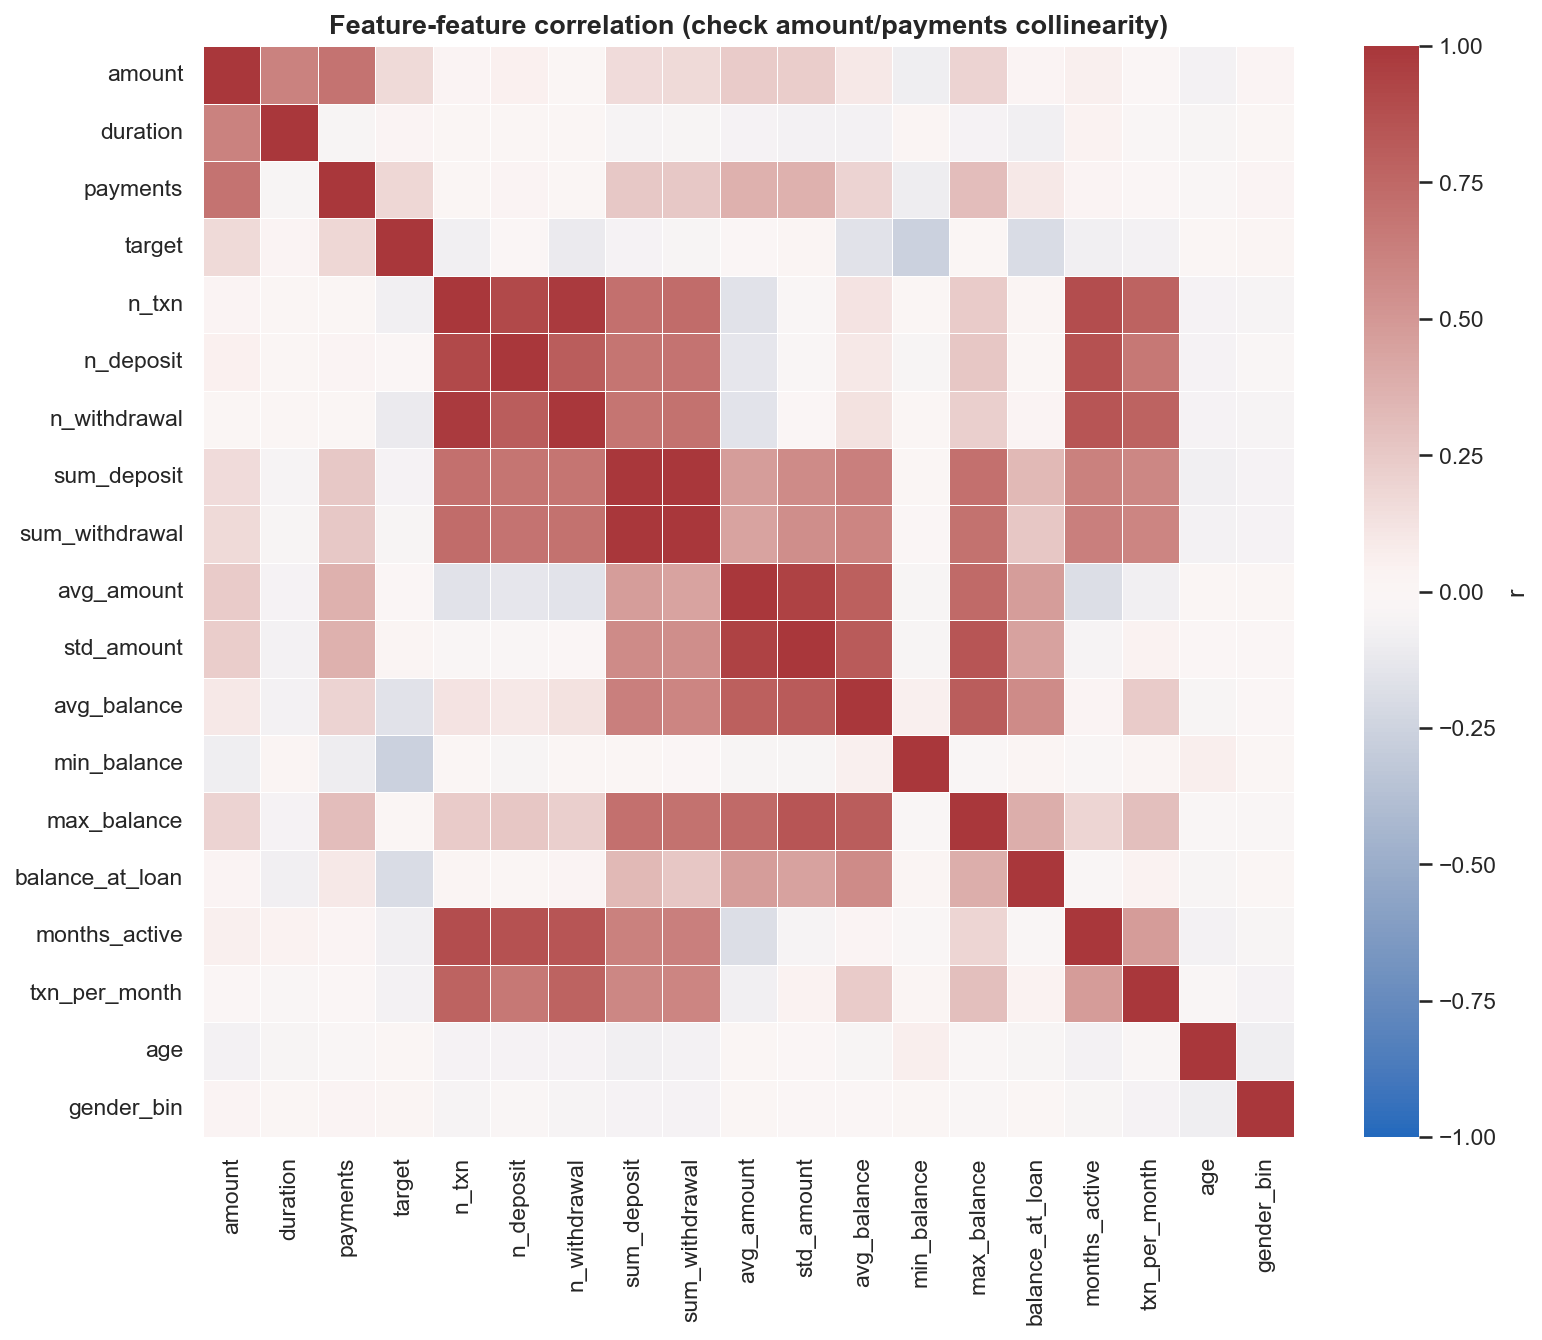
\includegraphics[width=0.85\textwidth]{corr_full.png}
    \caption{Correlation matrix of the numeric features. The cash-flow pair is nearly duplicated, and loan amount tracks monthly payment.}
    \label{fig:corr-full}
\end{figure}

The redundancy has a practical consequence for interpretation. When two features carry almost the same information, a tree can split on either one, and the reported importance can move between them across runs. The feature importance discussion in Chapter~\ref{ch:models} therefore groups related variables rather than treating each score as a separate causal effect.

\section{Loan Size Relative to Balance}
\label{sec:risk-quadrant}

The two strongest themes in the univariate analysis are balance level and loan size. Figure~\ref{fig:risk-quadrant} combines them. Loans are split at the median pre-loan balance of about 38,500 and the median loan amount of about 116,900. The four cells have very different default rates.

\begin{table}[H]
    \centering
    \caption{Default rate by pre-loan balance and loan amount, split at the respective medians.}
    \label{tab:risk-quadrant}
    \begin{tabular}{@{}llr@{}}
        \toprule
        \textbf{Balance} & \textbf{Loan amount} & \textbf{Default rate} \\
        \midrule
        High & Low & 4.9\% \\
        High & High & 6.7\% \\
        Low & Low & 10.1\% \\
        Low & High & 23.3\% \\
        \bottomrule
    \end{tabular}
\end{table}

The highest-risk cell is the borrower with a below-median balance asking for an above-median loan. Its default rate of 23.3\% is more than double the base rate and roughly five times the rate in the high-balance, low-amount cell. The pattern is intuitive: the loan is large relative to the buffer the account has shown. It also suggests a simple screening rule that does not require a model, which is useful as a sanity check on whatever the classifiers learn.

\begin{figure}[H]
    \centering
    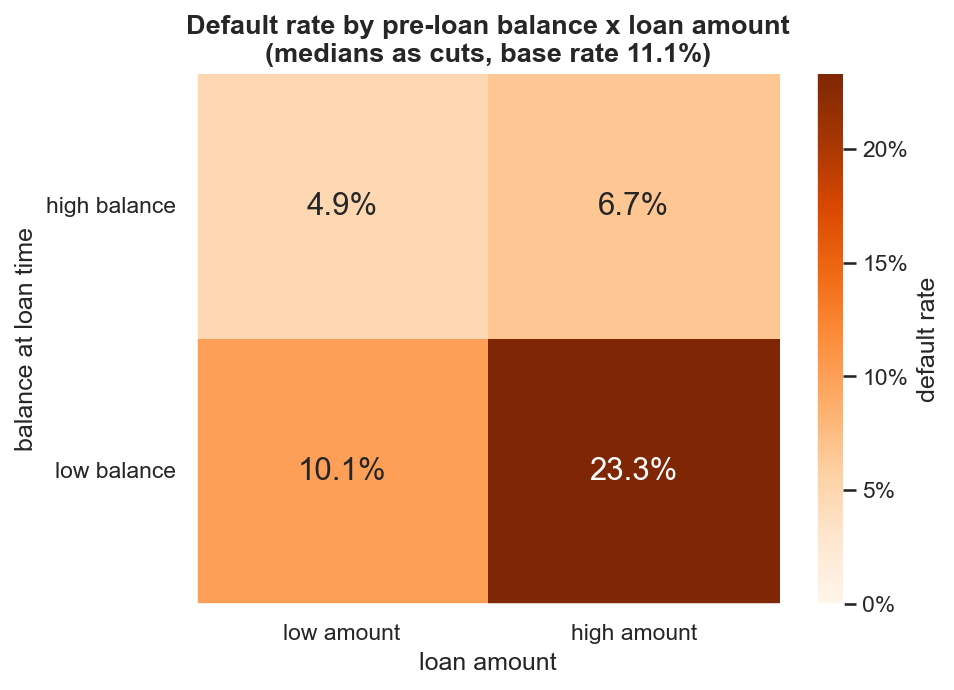
\includegraphics[width=0.62\textwidth]{risk_quadrant.png}
    \caption{Default rate by balance and loan amount. The low-balance, high-amount quadrant has the highest risk.}
    \label{fig:risk-quadrant}
\end{figure}

\section{Behavioural Segments}
\label{sec:segments}

A KMeans clustering with two groups was fitted on the behavioural and loan variables, with the target excluded. The silhouette score of 0.29 is modest, so the segments should be read as a coarse summary rather than as natural kinds. Figure~\ref{fig:segments-scatter} shows the separation in the balance and activity space, and Table~\ref{tab:segment-profiles} gives the profiles.

\begin{table}[H]
    \centering
    \caption{Profiles of the two behavioural segments. The target was not used to form the clusters.}
    \label{tab:segment-profiles}
    \begin{tabular}{@{}lrrrrr@{}}
        \toprule
        \textbf{Segment} & \textbf{Loans} & \textbf{Median txns} & \textbf{Mean balance} & \textbf{Txns/month} & \textbf{Default rate} \\
        \midrule
        0 & 421 & 54 & 37,200 & 5.2 & 12.4\% \\
        1 & 261 & 116 & 52,400 & 6.9 & 9.2\% \\
        \bottomrule
    \end{tabular}
\end{table}

Segment 0 is the larger, quieter group: fewer transactions, lower average balance, and a default rate of 12.4\%. Segment 1 is more active and holds a higher balance, with a default rate of 9.2\%. The direction is sensible, but the overlap is substantial. Activity alone does not separate the classes cleanly, which is consistent with the weak univariate correlation of \texttt{txn\_per\_month}. The segment label is useful for describing the portfolio, not for deciding a loan.

\begin{figure}[H]
    \centering
    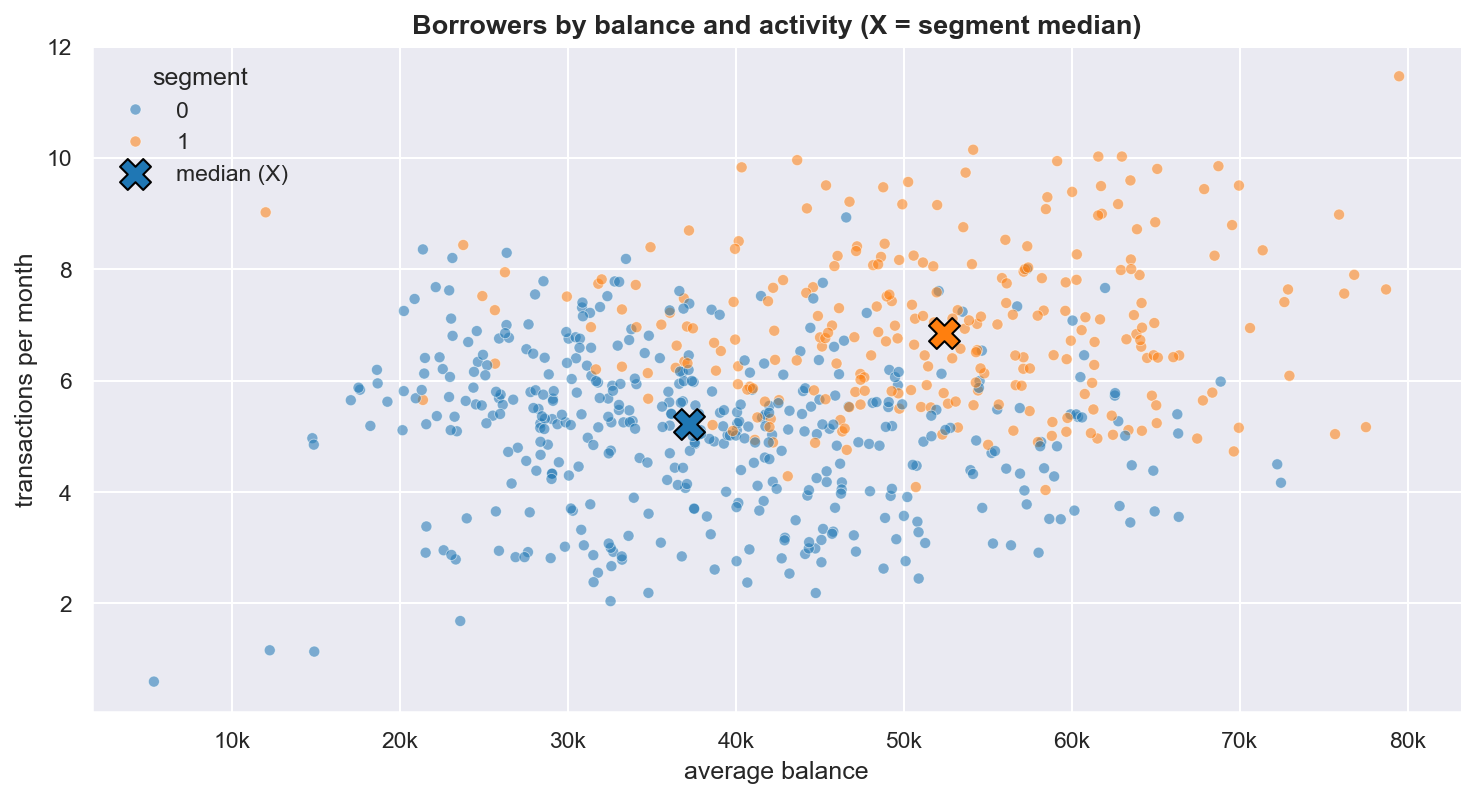
\includegraphics[width=0.9\textwidth]{segments_scatter.png}
    \caption{Loans in the two behavioural segments, plotted in the activity and balance space.}
    \label{fig:segments-scatter}
\end{figure}

\begin{figure}[H]
    \centering
    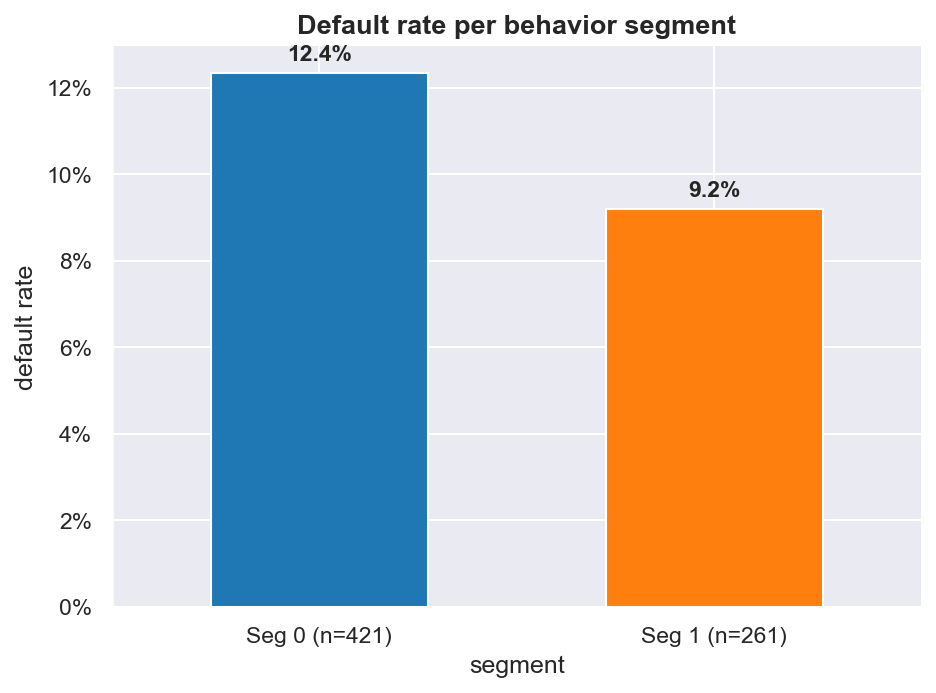
\includegraphics[width=0.62\textwidth]{segments_default.png}
    \caption{Default rate by segment. The quieter, lower-balance segment has the higher rate, but the difference is modest.}
    \label{fig:segments-default}
\end{figure}

\section{Summary of Findings}
\label{sec:eda-summary}

The exploratory work supports five conclusions that carry into the modelling chapter.

\begin{itemize}
    \item Balance history is the main behavioural axis. \texttt{min\_balance} and \texttt{balance\_at\_loan} have the strongest correlations with default, and their distributions separate visibly.
    \item Loan size matters in combination with balance. The low-balance, high-amount quadrant reaches a 23.3\% default rate, far above the 11.14\% base rate.
    \item Age and gender carry little signal. Their correlations are near zero and the age distribution shows no high-risk band.
    \item Activity volume is weak on its own. Transaction frequency is similar across classes, and the two clusters differ by only about three percentage points in default rate.
    \item Collinearity is present but manageable. The cash-flow pair is nearly duplicated, and the balance features overlap; interpretation should focus on groups of related variables.
\end{itemize}

These findings set expectations for the classifiers. A model should improve on the base rate mainly by using balance and loan burden, should not gain much from demographics, and should be judged on its ability to catch the small default class rather than on overall accuracy.
